\section{Loss Normalization and Task Performance}
\label{sec:normalization}

\subsection{Equal domain weights do not remove response-length weighting}

Sampling equal numbers of prompts per domain does not give each domain equal weight in the training loss, because student response lengths differ by domain. With token-level normalization over the full batch (GT), domains with longer responses receive more loss weight. Domain-token normalization (DT) fixes each domain's weight to $\lambda_d$ but still assigns longer responses more weight within that domain. Domain-response normalization (DR) also fixes the domain weights and gives equal weight to each response's mean loss. Domain balancing and within-domain loss normalization are therefore separate design choices, even with a fixed prompt mixture.

This difference changes the gradient whenever response length correlates with the response gradient. Write $g_i=\nabla_\theta\ell_i$, and let $\bar g_d$ and $\bar T_d$ denote the mean response gradient and response length within domain $d$. The token-weighted domain gradient satisfies
\begin{equation}
\frac{\sum_{i\in\mathcal B_d}T_i g_i}{\sum_{i\in\mathcal B_d}T_i}
=\bar g_d+\frac{\operatorname{Cov}_d(T,g)}{\bar T_d}.
\label{eq:weighting}
\end{equation}
The covariance term measures the effect of weighting response gradients by length. DT retains this term; DR uses $\bar g_d$ alone. Multiplying each domain's GT loss contribution by its target weight $\lambda_d$ divided by its observed token share gives DT exactly, as in Open-MOPD \citep[Section~4.1, Eq.~(8)]{gao2026openmopddiagnosingfixingcapability}. Thus correcting unequal domain token counts still leaves a choice between token-level and sequence-level normalization within each domain. Appendix~\ref{app:normalization} gives the derivation.

\subsection{Similar I64 endpoint scores despite different loss weights}

\paragraph{Training and evaluation.}
We train a Qwen3-1.7B student with four frozen teachers for mathematics, code, instruction following, and science. The three I64 configurations differ only in GT, DT, or DR loss normalization. They use the same initialization, teachers, prompt schedule, and optimizer settings, with 16 prompts per domain at each update. We evaluate MATH-500, a fixed LiveCodeBench subset, IFBench, and GPQA Diamond through update 500 and report their equally weighted mean. Appendix~\ref{app:setup} gives the training and scoring protocol.

\paragraph{Correcting a threefold loss-weight imbalance changes little at the I64 endpoint.}
Mathematics and instruction following each receive 25\% of prompts but account for 44.05\% and 14.98\% of GT's valid response tokens in the first 50 batches. GT therefore assigns mathematics nearly three times as much loss weight as instruction following, whereas DT and DR fix both at 25\% (Figure~\ref{fig:normalization_capability}a). Despite this difference, the update-500 four-domain scores are $38.58\pm0.75$\% (DR), $38.71\pm0.80$\% (DT), and $38.64\pm0.80$\% (GT), reported as mean $\pm$ standard deviation over three training seeds. The 0.14-percentage-point range between means is smaller than the 0.75--0.80-point seed standard deviations. The preferred rule varies with the task and checkpoint: all three improve mathematics and instruction following toward teacher performance, retain a code performance gap, and start near the science teacher's GPQA score (Figure~\ref{fig:normalization_capability}). Equal domain loss weights therefore do not consistently improve the final mean score in this I64/Adam setting.

\begin{figure}[t]
\centering
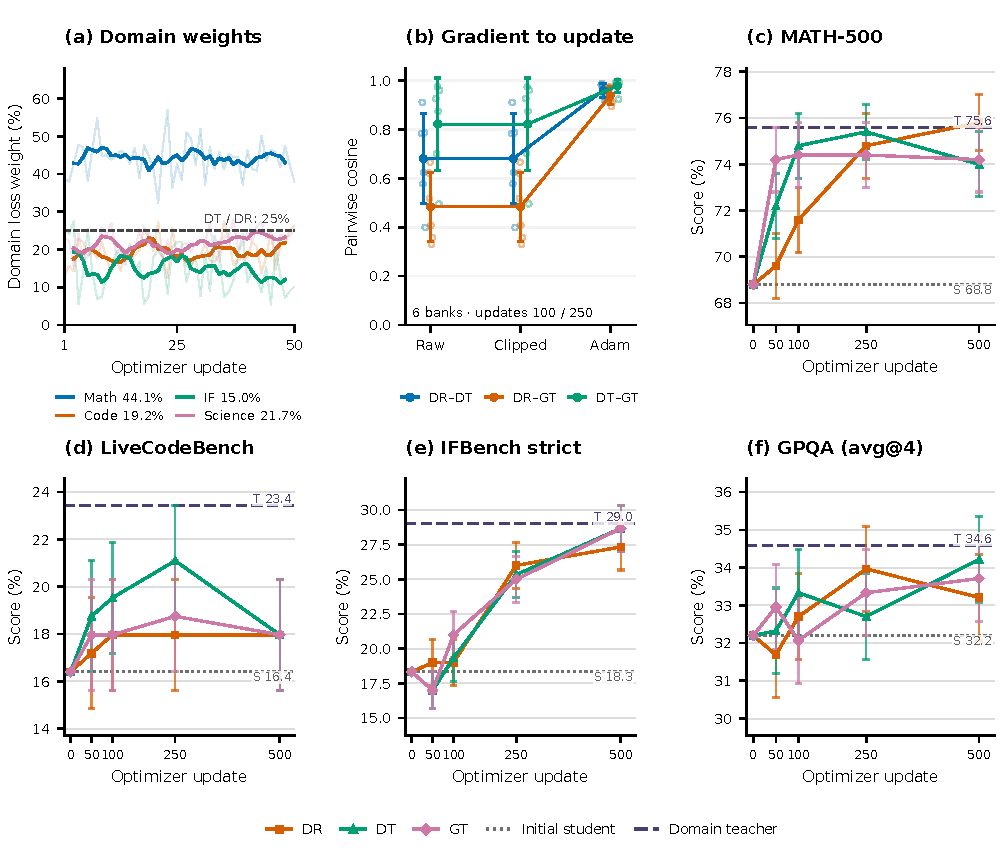
\includegraphics[width=\linewidth]{figures/nine_panel_20260914/section3_normalization.pdf}
\caption{Loss weighting, optimizer mediation, and task capability trajectories.
(a) GT domain loss weights across the first 50 updates: faint lines are individual batches, bold lines are five-batch moving averages, and legend values are arithmetic means over all 50 batches. DT and DR each fix domain weights at 25\%.
(b) Three reduction pairs before clipping, after clipping, and after a shared saved-state Adam update. Small open points are six fixed banks at updates 100/250; lines and error bars show their mean and sample standard deviation.
(c--f) GT/DT/DR scores on MATH-500, LiveCodeBench, IFBench strict, and GPQA (avg@4), with initial-student (S) and domain-teacher (T) references. Points and error bars retain the original means and sample standard deviations, computed from measured seed-42 scores and estimated seed-43/44 scores. The authors report agreement with subsequent three-seed experiments; the retained estimates are not independently verified measurements. Updates use a linear axis. Appendix Figure~\ref{fig:normalization_aggregate_support} gives the four-domain mean and worst-domain change.}
\label{fig:normalization_capability}
\end{figure}


\paragraph{Normalization changes PG/SGD endpoint scores by 1.07 points.}
In the seed-42 endpoint comparison, the four-domain score range between normalization rules is 0.33 points for PG/Adam and 1.07 points for PG/SGD, compared with 0.14 points for I64/Adam (Table~\ref{tab:completed_endpoints}). PG/SGD favors DR over GT by 1.07 points, while PG/Adam favors GT over DR by 0.07 points. The small differences under I64/Adam therefore do not establish that normalization is unimportant for other training configurations. All ten configurations improve the initial four-domain mean from 33.93\% to 38.03--39.46\%. These results use one training seed, unlike the three-seed I64 summary above. The SGD runs also use a different learning rate and deployment, so their higher scores do not isolate the effect of the optimizer or establish a training-efficiency advantage. Appendix~\ref{app:completed_results} reports the separate test-set evaluation.

% Estimated paired intervals: experiments/table1_paired_estimates_20260918/estimate_intervals.py.
\begin{table}[t]
\centering\small
\setlength{\tabcolsep}{3.5pt}
\caption{\textbf{Task gains coexist with domain-level trade-offs.} Joint-training endpoint scores (\%); Mean weights domains equally. PG: sampled-token supervision; I16/I64: top-16/top-64 intersection supervision. DR/DT: equal domain weights with response/token averaging; GT: global token averaging. $\Delta$ is the mean difference from PG-DR/Adam (percentage points). Brackets give model-based paired 95\% intervals (Appendix~\ref{app:capability_uncertainty}).}
\label{tab:completed_endpoints}
\begin{tabular}{lrrrrrr}
\toprule
Configuration & MATH-500 & Code & IF & GPQA & Mean & $\Delta$ [95\% interval] \\
\midrule
Initial student & 68.80 & 16.41 & 18.33 & 32.20 & 33.94 & $-4.68$ [-6.42, -2.93] \\
\midrule
\multicolumn{7}{l}{\textit{Adam}} \\
PG-DR & 73.20 & 18.27 & 27.00 & 35.97 & 38.61 & Reference \\
PG-DT & 73.20 & 19.24 & 27.00 & 34.96 & 38.60 & $-0.01$ [-1.45, 1.43] \\
PG-GT & 76.20 & 17.92 & 27.33 & 32.94 & 38.60 & $-0.01$ [-1.44, 1.42] \\
I16-DR & 75.40 & 17.75 & 27.00 & 35.46 & 38.90 & $+0.29$ [-1.15, 1.73] \\
I64-DR & 75.80 & 18.30 & 27.33 & 34.71 & 39.04 & $+0.43$ [-1.01, 1.86] \\
I64-DT & 74.00 & 18.86 & 28.67 & 35.22 & 39.19 & $+0.58$ [-0.87, 2.02] \\
I64-GT & 74.20 & 19.80 & 28.67 & 33.41 & 39.02 & $+0.41$ [-1.03, 1.85] \\
\midrule
\multicolumn{7}{l}{\textit{SGD}} \\
PG-DR & 76.40 & 19.53 & 28.33 & 35.59 & 39.96 & $+1.35$ [-0.09, 2.79] \\
PG-DT & 75.20 & 20.31 & 28.33 & 33.90 & 39.44 & $+0.83$ [-0.61, 2.26] \\
PG-GT & 75.00 & 19.26 & 25.33 & 34.71 & 38.58 & $-0.04$ [-1.47, 1.40] \\
\bottomrule
\end{tabular}
\par\vspace{2pt}
\end{table}


\subsection{Adam reduces directional differences between normalization rules}

\paragraph{Different gradients produce more similar Adam updates.}
I64 gradient cosines average 0.680 (DR--DT), 0.483 (DR--GT), and 0.822 (DT--GT) on six fixed response batches at joint-PG checkpoints 100 and 250. These comparisons hold the student weights, responses, token masks, and teacher scores fixed, so the directional differences come from loss normalization. In particular, the DR--DT comparison shows that equal domain weights do not eliminate the effect of response-length weighting. Applying each gradient from an identical copy of the saved Adam first- and second-moment estimates raises the corresponding FP32 update cosines to 0.960, 0.939, and 0.979. The resulting parameter updates are therefore much more similar in direction than the gradients used to compute them.

\paragraph{Gradient clipping changes magnitude, not direction.}
Global norm clipping leaves all three pairwise gradient cosines unchanged. Its frequency nevertheless differs sharply during training: DR is clipped on all 500 updates and retains a median 9.3\% of the gradient norm, whereas DT and GT are clipped on 46.2\% and 15.0\% of updates, respectively (Figure~\ref{fig:normalization_interventions}a). Clipping alone therefore cannot explain the increase in update cosine under Adam. Resetting Adam's moment estimates also changes the update norms (Figure~\ref{fig:normalization_interventions}b), showing that the saved optimizer state affects update magnitude as well as direction.

\paragraph{One-step loss changes also depend on the optimizer state.}
After one Adam step from the same saved moment estimates, the three normalization rules produce similar changes in held-out reverse KL relative to the variation between response batches (Figure~\ref{fig:normalization_interventions}c). When SGD steps are rescaled to match each rule's Adam update norm, the differences between rules are larger: all three reduce mean held-out KL at update 100 but increase it at update 250. These measurements concern the immediate effect of one update on fixed held-out responses. They do not account for the complete training trajectories, in which each student generates different responses and accumulates different Adam moments. Appendix~\ref{app:fixed_batch_normalization} gives the one-step protocol and gradient comparisons; Figure~\ref{fig:normalization_ci} reports paired task-score contrasts.

\begin{figure}[t]
\centering
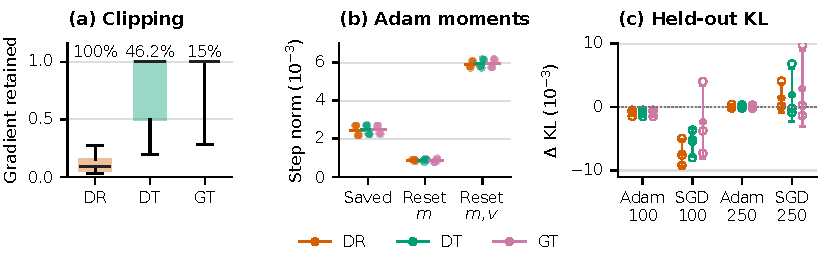
\includegraphics[width=\linewidth]{figures/added_control_figures_20260914/normalization_interventions.pdf}
\caption{Optimizer interventions.
(a) Gradient fraction retained over 500 updates per reduction; labels give clipping rates, boxes the interquartile range, and whiskers the 5th--95th percentiles.
(b) FP32 step norms across six banks; bars show means.
(c) Immediate held-out reverse-KL changes under saved Adam and norm-matched SGD; lower is better. Open points denote banks; filled points and error bars show mean $\pm$ sample SD.}
\label{fig:normalization_interventions}
\end{figure}


\FloatBarrier
